\chapter{Extremal Kerr black hole}
\label{s:exk}

\minitoc

\section{Introduction}

The Kerr solution of Einstein equation has been introduced in Sec.~\ref{s:ker:Kerr_solution};
it depends on two parameters: the mass $m > 0$ and the spin parameter
$a \geq 0$.
In Chaps.~\ref{s:ker}--\ref{s:gik}, we have considered the Kerr solution with $0<a<m$,
while the case $a=0$ (Schwarzschild solution) was the subject of Chaps.~\ref{s:sch}--\ref{s:max}.
Here we focus on the case $a=m$, which is called the \emph{extremal Kerr spacetime}.
This corresponds to the highest value of $a$
for which the Kerr solution describes a black hole.
Indeed, for $a> m$, the Kerr metric is still an exact
solution of the vacuum Einstein equation, but it describes a \emph{naked singularity}\index{naked singularity} (cf. Sec.~\ref{s:max:naked_sing}):
the ring curvature singularity is not hidden by any horizon to asymptotic observers.
Moreover, as we going to see, the Kerr spacetime with $a=m$ has many properties that are not
shared by Kerr spacetimes with $a<m$. In particular, the black hole event horizon is
\emph{degenerate}, in the sense defined in Sec.~\ref{s:neh:classif_KH}, i.e. it has a
vanishing surface gravity $\kappa$. Besides, the maximal analytic extension is simpler than
that of the Kerr spacetime with $a<m$.
Another specific property of the extremal Kerr spacetime
regards the geometry near the horizon: it admits an enlarged
symmetry group, which is generated
by four independent Killing vectors,
instead of two for the geometry of
the global solution.


%%%%%%%%%%%%%%%%%%%%%%%%%%%%%%%%%%%%%%%%%%%%%%%%%%%%%%%%%%%%%%%%%%%%%%%%%%%%%%%

\section{Definition and basic properties}

\subsection{The extremal Kerr solution}

Let us consider the manifold $\R^2\times\SS^2$ described by
coordinates $(\ti, r, \th,\tph)$ such that $(\ti,r)$ cover $\R^2$
and $(\th,\tph)$ are standard spherical coordinates on $\SS^2$.
The \defin{extremal Kerr spacetime}\index{extremal!Kerr spacetime}\index{Kerr!extremal -- spacetime}
of mass $m>0$ is defined as the pair $(\M, \w{g})$ where the manifold $\M$ is the following open subset of $\R^2\times\SS^2$:
\be \label{e:exk:def_M}
 \M := \R^2\times\SS^2 \setminus \ring
\ee
with
\be \label{e:exk:def_ring}
    \ring := \left\{ p \in \R^2\times\SS^2,
        \quad r(p) = 0 \ \mbox{and}\ \th(p) = \frac{\pi}{2} \right\} ,
\ee
and the metric $\w{g}$ has the following expression in terms of the coordinates
$(x^{\tilde{\alpha}}) = (\ti, r, \th,\tph)$:
\be \label{e:exk:metric_Kerr_3p1}
    \encadre{
    \begin{array}{ll}
    g_{\tilde{\mu}\tilde{\nu}}\, \D x^{\tilde{\mu}} \, \D x^{\tilde{\nu}}   = &
    \displaystyle - \left( 1 - \frac{2m r}{\rho^2} \right)  \D \ti^2
    + \frac{4m r}{\rho^2} \D\ti\, \D r
    - \frac{4 m^2  r \sin^2\th}{\rho^2} \,  \D \ti\, \D\tph \\[2ex]
    &\displaystyle  + \left( 1 + \frac{2m r}{\rho^2} \right) \D r^2
     - 2 m \left( 1 + \frac{2m r}{\rho^2} \right) \sin^2\th \, \D r\, \D \tph \\[2ex]
    & \displaystyle + \rho^2 \D \th^2
    + \left( r^2 + m^2 + \frac{2 m^3 r \sin^2\th}{\rho^2} \right)
    \sin^2\th \, \D \tph^2 ,
    \end{array}
    }
\ee
with
\be
    \rho^2 := r^2 + m^2\cos^2\th .
\ee
In this context, the coordinates $(x^{\tilde{\alpha}}) = (\ti, r, \th,\tph)$
are called
\defin{Kerr coordinates}\index{Kerr!coordinates}
and we recognize in (\ref{e:exk:metric_Kerr_3p1}) the limit $a\to m$ of
expression (\ref{e:ker:metric_Kerr_3p1}) for the Kerr metric with $a< m$.

The metric (\ref{e:exk:metric_Kerr_3p1}) is regular
in all $\M$, since the components $g_{\tilde{\alpha}\tilde{\beta}}$ are singular only
for $\rho=0$, i.e. for $r=0$ and $\th=\pi/2$, which defines  the set $\ring$ that has precisely been excluded from $\M$ by
the definition (\ref{e:exk:def_M}). The Kretschmann curvature
invariant\index{Kretschmann scalar! of Kerr metric} $K := R_{\mu\nu\rho\sigma} R^{\mu\nu\rho\sigma}$
is given by Eq.~(\ref{e:ker:Kretschmann}) with $a=m$; it diverges for $\rho\to 0$. Therefore, as
for the Kerr spacetime with $a<m$ (cf. Sec.~\ref{s:ker:singularities}), we shall call $\ring$ the \defin{ring singularity}\index{ring!singularity}\index{singularity!ring --}
of the extremal Kerr spacetime. Note that, formally, it is not part of the spacetime manifold
$\M$ [cf. Eq.~(\ref{e:exk:def_M})].

Moreover, the Ricci tensor of the metric (\ref{e:exk:metric_Kerr_3p1}) is identically zero in all
$\M$ (see the notebook~\ref{s:sam:Kerr_extremal} for the computation). Hence, we have:
\begin{greybox}
The metric $\w{g}$ of the extremal Kerr spacetime is a solution of Einstein equation\index{Einstein!equation} (\ref{e:fra:Einstein_eq})
in vacuum ($\w{T}=0$) and with a vanishing cosmological constant ($\Lambda=0$).
\end{greybox}

The inverse metric is
\be \label{e:exk:inv_met_3p1}
    g^{\tilde{\alpha}\tilde{\beta}} = \left(
    \begin{array}{cccc}
    - \left( 1 + \frac{2m r}{\rho^2} \right) & \frac{2m r}{\rho^2} & 0 & 0 \\[1ex]
    \frac{2m r}{\rho^2} & \frac{(r-m)^2}{\rho^2} & 0 & \frac{m}{\rho^2} \\[1ex]
    0 & 0 &\frac{1}{\rho^2} & 0 \\[1ex]
    0 & \frac{m}{\rho^2} & 0 & \frac{1}{\rho^2\sin^2\th}
    \end{array}
    \right) .
\ee


\subsection{Boyer-Lindquist coordinates}

For $a<m$, the Kerr manifold $\M$ has been split in three open regions,
$\M_{\rm I}$, $\M_{\rm II}$ and $\M_{\rm III}$,  separated by the two Killing
horizons $\Hor$ and $\Hor_{\rm in}$
[cf. Eqs.~(\ref{e:ker:def_M_Kerr_spacetime}) and (\ref{e:ker:def_M_BL})].
Since $\Hor$ was defined by $r=r_+:=m + \sqrt{m^2 - a^2}$ [Eq.~(\ref{e:ker:def_H})]
and $\Hor_{\rm in}$
by $r=r_-:=m - \sqrt{m^2 - a^2}$ [Eq.~\ref{e:ker:def_H_in})],
we notice that
$r_+ = r_- = m$ in the limit $a\to m$.
This implies that $\Hor$ and $\Hor_{\rm in}$ coincide when $a\to m$ and the region
$\M_{\rm II}$, which is bounded by $\Hor$ and $\Hor_{\rm in}$, disappears.
Accordingly, we shall split the extremal Kerr manifold $\M$ in two open regions only,
$\M_{\rm I}$ and $\M_{\rm III}$, separated by a single hypersurface $\Hor$:
\be
    \encadre{\M = \M_{\rm I} \cup \Hor \cup \M_{\rm III} },
\ee
with
\begin{subequations}
\begin{align}
    \M_{\rm I} & := \left\{ p \in \M, \quad r(p) > m \right\} \\
    \Hor & := \left\{ p \in \M, \quad r(p) = m \right\} \label{e:exk:def_H}\\
    \M_{\rm III} & := \left\{ p \in \M, \quad r(p) < m \right\} .
\end{align}
\end{subequations}
\begin{remark}
We are using the notation $\M_{\rm III}$ for the ``second'' region, and not $\M_{\rm II}$,
to be consistent with Chaps.~\ref{s:ker}--\ref{s:gik}, i.e. with
the limit $a\to m$ of the results obtained in these chapters.
\end{remark}
The quadratic polynomial in $r$ introduced in Chap.~\ref{s:ker},
$\Delta=r^2 - 2 m r + a^2 = (r - r_+)(r - r_-)$, reduces to $\Delta = (r - m)^2$
in the limit $a\to m$. Its double root, $r=m$, defines the hypersurface $\Hor$.


In the region $\M_{\rm BL}:= \M \setminus \Hor = \M_{\rm I} \cup \M_{\rm III}$, one may introduce
the \defin{Boyer-Lindquist coordinates}\index{Boyer-Lindquist coordinates}
$(t,r,\th,\ph)$ such that $(r,\th)$ are the same coordinates as in
Kerr coordinates, while $t$ and $\ph$ are related to the Kerr coordinates
$\ti$, $r$ and $\tph$ by
\begin{subequations}
\label{e:exk:3p1_Kerr_to_BL}
\begin{align}
    t & = \ti +  \frac{2m^2}{r - m} - 2m \ln \left| \frac{r - m}{m} \right|
            \label{e:exk:3p1_Kerr_to_BL_t} \\
    \ph & = \tph + \frac{m}{r - m} . \label{e:exk:3p1_Kerr_to_BL_ph}
\end{align}
\end{subequations}
Differentiating these relations leads to
\be \label{e:exk:dt_dph}
    \D \ti = \D t  + \frac{2m r}{(r- m)^2} \, \D r
    \qand
    \D \tph = \D \ph + \frac{m}{(r - m)^2 } \, \D r .
\ee
\begin{remark}
The differential relations (\ref{e:exk:dt_dph}) can be obtained immediately
by substituting $a$ by $m$ in relations (\ref{e:ker:Kerr_3p1_BL}). However, to get the integrated
relations (\ref{e:exk:3p1_Kerr_to_BL}) from their $a<m$ analog
(\ref{e:ker:Kerr_3p1_BL_int}), one must perform an expansion in $\veps := \sqrt{m^2 - a^2}/m$,
taking into account that $r_\pm = m(1\pm\veps)$. One obtains then
(\ref{e:exk:3p1_Kerr_to_BL_t})
up to the additive constant $(2\ln 2) m$, while (\ref{e:exk:3p1_Kerr_to_BL_ph}) is recovered in the same form.
\end{remark}
It follows from the transformations (\ref{e:exk:3p1_Kerr_to_BL}) that
the Boyer-Lindquist coordinate frame $(\wpar_\alpha)$ and the Kerr coordinate frame $(\wpar_{\tilde{\alpha}})$ are related by\footnote{See also the limit $a\to m$ of Eq.~(\ref{e:ker:frame_Kerr3p1_BL}).}
\begin{subequations}
\label{e:exk:frame_BL_Kerr3p1}
\begin{align}
    & \wpar_t  = \wpar_\ti  \\
    & \wpar_r = \wpar_{\tilde r} + \frac{2mr}{(r-m)^2} \wpar_\ti
                        + \frac{m}{(r-m)^2} \wpar_\tph \\
    & \wpar_\th = \wpar_\th \\
    & \wpar_\ph = \wpar_{\tph} .
\end{align}
\end{subequations}
Note that, as in Chap.~\ref{s:ker}, we have denoted by $\wpar_{\tilde r}$ the second vector of the
coordinate frame associated to the Kerr coordinates
$(x^{\tilde{\alpha}}) = (\ti, r, \th,\tph)$, in order to distinguish it from
the coordinate vector
$\wpar_r$ of the Boyer-Lindquist coordinates
$(x^\alpha) = (t,r,\th,\ph)$.

\begin{figure}
\centerline{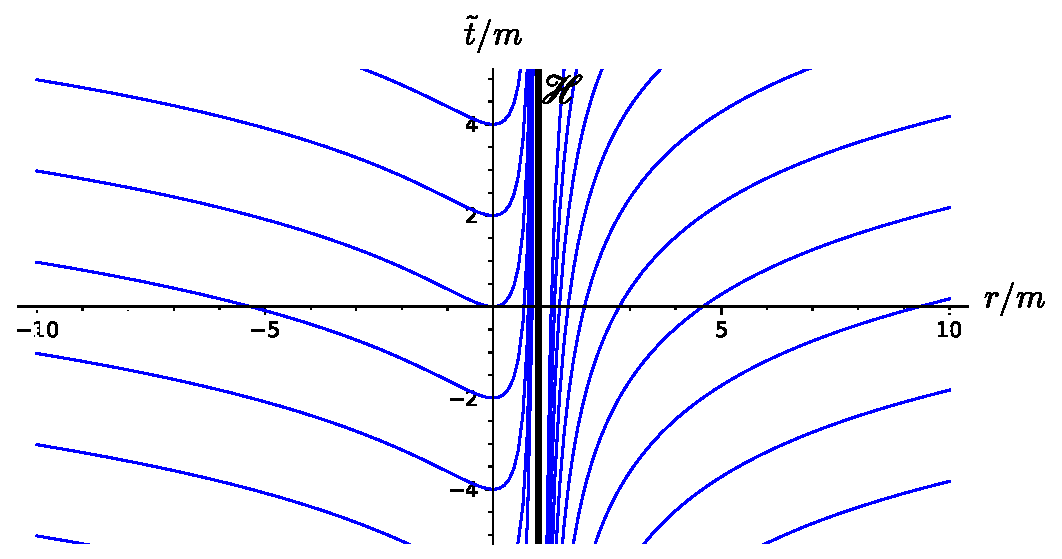
\includegraphics[width=0.7\textwidth]{exk_BL_slicing.pdf}}
\caption[]{\label{f:exk:BL_slicing} \footnotesize
Trace of the hypersurfaces of constant Boyer-Lindquist time $t$ in the plane
$(\tilde{t}, r)$.
\textsl{[Figure generated by the notebook \ref{s:sam:Kerr_extremal}]}
}
\end{figure}

The metric components $(g_{\alpha\beta})$ with respect to the Boyer-Lindquist coordinates $(x^\alpha) = (t,r,\th,\ph)$ are given by
\be \label{e:exk:metric_BL}
    \encadre{
    \begin{array}{ll}
    g_{\mu\nu}\,  \D x^\mu \D x^\nu  = &
    \displaystyle - \left( 1 - \frac{2m r}{\rho^2} \right) \, \D t^2
    - \frac{4 m^2  r \sin^2\th}{\rho^2} \,  \D t\, \D\ph
    + \frac{\rho^2}{(r-m)^2} \, \D r^2  \\[2ex]
    & \displaystyle + \rho^2 \D \th^2
    + \left( r^2 + m^2 + \frac{2 m^3 r \sin^2\th}{\rho^2} \right)
    \sin^2\th \, \D \ph^2 .
    \end{array}
    }
\ee
This expression can be obtained either by taking the limit $a\to m$ of Eq.~(\ref{e:ker:metric_BL})
or by using (\ref{e:exk:dt_dph}) to substitute $\D\ti$ and $\D\tph$ in Eq.~(\ref{e:exk:metric_Kerr_3p1}).
We note that $g_{rr}\to +\infty$ when $r\to m$, which reflects the singularity of Boyer-Lindquist
coordinates on $\Hor$ and explains why the latter was excluded in the definition
of $\M_{\rm BL}$. This singularity is clearly apparent in the coordinate transformations
(\ref{e:exk:3p1_Kerr_to_BL}), as well as in the spacetime slicing by the
hypersurfaces $t=\mathrm{const}$ depicted in Fig.~\ref{f:exk:BL_slicing}: the slices accumulate
onto $\Hor$, without crossing it, so that the points on $\Hor$ do not belong to any
hypersurface $t=\mathrm{const}$. That the $t=\mathrm{const}$ hypersurfaces do not provide a
regular slicing of the extremal Kerr spacetime $(\M,\w{g})$ is also manifest on
the Carter-Penrose diagram shown in Fig.~\ref{f:exk:CPdiag_BL}.

The inverse metric $\w{g}^{-1}$ has the following components in Boyer-Lindquist coordinates
(cf. the limit $a\to m$ of Eq.~(\ref{e:ker:inv_met_BL})):
\be \label{e:exk:inv_met_BL}
    g^{\alpha\beta} = \left(
    \begin{array}{cccc}
    - \frac{1}{(r-m)^2}
    \left( r^2 + m^2 + \frac{2 m^3 r \sin^2\th}{\rho^2} \right)
     & 0 & 0 & -\frac{2 m^2 r}{\rho^2 (r-m)^2} \\[1ex]
    0 & \frac{(r-m)^2}{\rho^2} & 0 & 0 \\[1ex]
    0 & 0 &\frac{1}{\rho^2} & 0 \\[1ex]
    -\frac{2 m^2 r}{\rho^2 (r-m)^2} & 0 & 0 &
    \frac{1}{(r-m)^2\sin^2\th}\left(1 - \frac{2 m r}{\rho^2} \right)
    \end{array}
    \right) .
\ee

\subsection{Symetries}

The extremal Kerr metric (\ref{e:exk:metric_Kerr_3p1}) is stationary\footnote{Cf.
Sec.~\ref{s:sta:def_station} for the definition of \emph{stationary} and a discussion
about the terminology.} and axisymmetric. The corresponding isometry group is $\R\times\mathrm{SO}(2)$ and is generated
by two commuting Killing vectors $\w{\xi}$ and $\w{\eta}$. Both the Kerr coordinates and
the Boyer-Lindquist ones are adapted to the spacetime symmetries, i.e. $(\ti,\tph)$ and
$(t,\ph)$ are ignorable coordinates, as it is clear on the line elements (\ref{e:exk:metric_Kerr_3p1})
and (\ref{e:exk:metric_BL}). Accordingly, one can normalize the Killing vectors so that
\be \label{e:exk:Killing_vectors}
    \encadre{\w{\xi} = \wpar_{\ti} = \wpar_t}
    \qand
    \encadre{\w{\eta} = \wpar_{\tph} = \wpar_\ph} .
\ee

\begin{figure}
\centerline{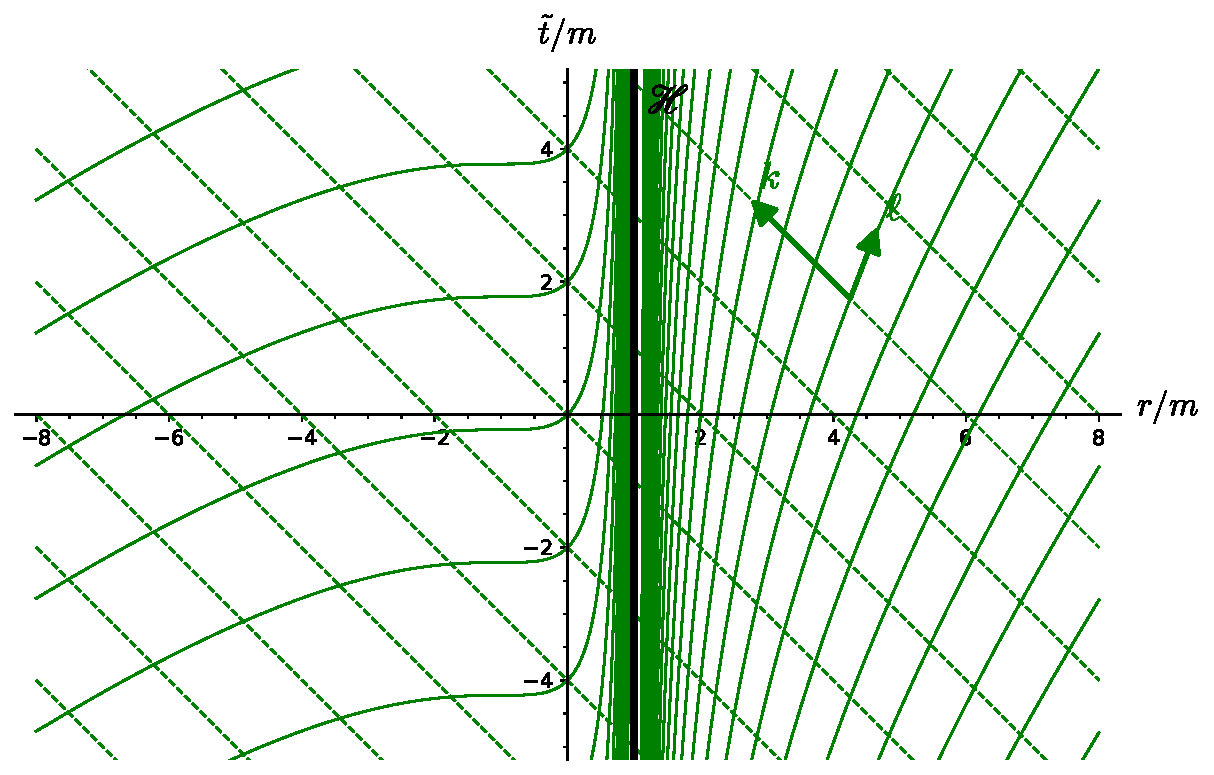
\includegraphics[width=0.8\textwidth]{exk_princ_null_geod.pdf}}
\caption[]{\label{f:exk:princ_null_geod} \footnotesize
Trace of the principal null geodesics in the plane
$(\tilde{t}, r)$. The dashed lines correspond to the
ingoing principal null geodesics $\Li^{\rm in}_{(v,\th,\tph)}$
and the solid curves to the
outgoing principal null geodesics $\Li^{\rm out,I}_{(u,\th,\tilde{\tph})}$
for $r>m$ and $\Li^{\rm out,III}_{(u,\th,\tilde{\tph})}$ for $r<m$.
\textsl{[Figure generated by the notebook \ref{s:sam:Kerr_extremal}]}
}
\end{figure}



\subsection{Principal null geodesics} \label{s:exk:princ_null_geod}

As discussed in Sec.~\ref{s:ker:principal_geod}, the Kerr spacetime is
endowed with two congruences of null geodesics tied to
the spacetime structure, as described by the Weyl conformal curvature tensor.
All the results of Sec.~\ref{s:ker:principal_geod} remain valid at the limit $a\to m$.
We can summarize them as follows:
\begin{greybox}
\begin{itemize}
\item The \defin{ingoing principal null geodesics} are the curves
\be
    \Li^{\rm in}_{(v,\th,\tph)}:\quad
        (v,\th,\tph) = \mathrm{const} \in \R\times[0,\pi]\times[0,2\pi), %]
\ee
where $v$ is the Kerr advanced time:
\be \label{e:exk:def_v}
    v := \ti + r = t  + r - \frac{2m^2}{r -m} + 2m\ln\left| \frac{r - m}{m} \right|.
\ee
Along any geodesic $\Li^{\rm in}_{(v,\th,\tph)}$, $-r$ is an affine parameter increasing towards the future;
the corresponding tangent vector is
\begin{subequations}
\begin{align}
 \w{k} & = \wpar_{\ti} - \wpar_{\tilde{r}} \label{e:exk:k_3p1_Kerr}\\
 \w{k} & = \frac{r^2 + m^2}{(r - m)^2} \, \wpar_t
            - \wpar_r + \frac{m}{(r - m)^2} \, \wpar_\ph
            \quad \mbox{in}\ \M\setminus\Hor .  \label{e:exk:k_BL}
\end{align}
\end{subequations}
\item The \defin{outgoing principal null geodesics} are the curves
\begin{subequations}
\begin{align}
  \mbox{in}\ \M_{\rm I} :&\quad \Li^{\rm out, I}_{(u,\th,\tilde{\tph})}:
    \quad   (u,\th,\tilde{\tph}) = \mathrm{const} \in \R\times[0,\pi]\times[0,2\pi), \\ %]
  \mbox{in}\ \M_{\rm III}:&\quad \Li^{\rm out, III}_{(u,\th,\tilde{\tph})}:
    \quad   (u,\th,\tilde{\tph}) = \mathrm{const} \in \R\times[0,\pi]\times[0,2\pi), \\ %]
 \mbox{on}\  \Hor: &\quad \Li^{{\rm out},\Hor}_{(\th,\psi)}:
    \quad  (\th,\psi) = \mathrm{const} \in [0,\pi]\times[0,2\pi),  %]
\end{align}
\end{subequations}
where $u$ is the Kerr retarded time:
\be \label{e:exk:def_u}
    u := \ti - r + \frac{4 m^2}{r - m} - 4 m \ln \left| \frac{r - m}{m} \right|
      = t  - r + \frac{2m^2}{r -m} - 2m\ln\left| \frac{r - m}{m} \right|
\ee
and $\tilde{\tph}$ and $\psi$ are defined by
\be \label{e:exk:def_ttph}
    \tilde{\tph} := \tph + \frac{2m}{r -m} = \ph + \frac{m}{r - m}
\ee
and
\be \label{e:exk:psi_tph_ti}
    \psi := \tph - \frac{\ti}{2m} .
\ee
Along the geodesics $\Li^{\rm out, I}_{(u,\th,\tilde{\tph})}$ and $\Li^{\rm out, III}_{(u,\th,\tilde{\tph})}$,
$r$ is an affine parameter increasing towards the future,
while along $\Li^{{\rm out},\Hor}_{(\th,\psi)}$, such an affine parameter is $\ti$. The tangent vector $\wl$ to the outgoing principal null geodesics
that coincides with the Killing vector $\w{\xi} + (2m)^{-1} \w{\eta}$ on $\Hor$ is
\begin{subequations}
\begin{align}
 \wl & = \frac{(r + m)^2}{2(r^2 + m^2)}\, \wpar_{\ti}
  + \frac{(r - m)^2}{2(r^2 + m^2)} \,  \wpar_{\tilde{r}}
  + \frac{m}{r^2 + m^2} \, \wpar_{\tph} \label{e:exk:ell_3p1_Kerr}\\
 \wl & =  \frac{1}{2}\, \wpar_t
            + \frac{(r - m)^2}{2(r^2 + m^2)} \,  \wpar_r
            + \frac{m}{2(r^2 + m^2)} \, \wpar_\ph
            \quad \mbox{in}\ \M\setminus\Hor . \label{e:exk:ell_BL}
\end{align}
\end{subequations}
\end{itemize}
\end{greybox}
\begin{proof}
The second equality in Eq.~(\ref{e:exk:def_v}) follows from Eq.~(\ref{e:exk:3p1_Kerr_to_BL_t}).
Equation~(\ref{e:exk:k_BL}) follows from Eq.~(\ref{e:exk:k_3p1_Kerr}) via Eq.~(\ref{e:exk:frame_BL_Kerr3p1}).
Equations~(\ref{e:exk:def_u}) and (\ref{e:exk:def_ttph}) are the integrated version of the system (\ref{e:ker:out_Kerr_Kerr_3p1}) with $a=m$. Equations~(\ref{e:exk:psi_tph_ti}), (\ref{e:exk:ell_3p1_Kerr})
and (\ref{e:exk:ell_BL}) are the $a=m$ versions of respectively
Eqs.~(\ref{e:ker:psi_tph_ti}), (\ref{e:ker:def_ell_outgoing}) and (\ref{e:ker:ell_BL}).
All the other statements follow from the limit $a\to m$ of results of Sec.~\ref{s:ker:principal_geod},
except for $\ti$ being an affine parameter along $\Li^{{\rm out},\Hor}_{(\th,\psi)}$, which
is peculiar to the extremal Kerr horizon and will
be proven in Sec.~\ref{s:exk:horizon}.
\end{proof}

The principal null geodesic congruences are depicted in terms of the $(\ti, r)$
coordinates in Fig.~\ref{f:exk:princ_null_geod}. Note that the outgoing geodesics
$\Li^{\rm out, I}_{(u,\th,\tilde{\tph})}$ and $\Li^{\rm out, III}_{(u,\th,\tilde{\tph})}$
tend to become tangent to $\Hor$ for $r\to m$; this agrees with $\Hor$ being
generated by some members of the outgoing principal null congruence, namely the geodesics
$\Li^{{\rm out},\Hor}_{(\th,\psi)}$, as we shall see in details in the next subsection.
Another view of the principal null geodesics is provided by the Carter-Penrose
diagram of $(\M,\w{g})$ shown in Fig.~\ref{f:exk:CPdiag_Kerr}, in which both
families of geodesics appear as straight lines.

\subsection{The degenerate horizon} \label{s:exk:horizon}

$\Hor$ is the hypersurface of $\M$ defined by $r=m$ [Eq.~(\ref{e:exk:def_H})]. Given
that the component $g^{rr} = (r - m)^2/\rho^2$ of the inverse metric with respect to Kerr coordinates
[Eq.~(\ref{e:exk:inv_met_3p1})] vanishes at $r=m$, we have
$g^{\tilde{\mu}\tilde{\nu}} \partial_{\tilde{\mu}} r \partial_{\tilde{\nu}} r = 0$ on $\Hor$,
which implies that the gradient $\vw{\nabla} r$
is a null vector there and that $\Hor$ is a null hypersurface.
Moreover, since the components of $\vw{\nabla} r$ are $\nabla^{\tilde{\alpha}} r = g^{\tilde{\alpha}r}$,
we read on Eq.~(\ref{e:exk:inv_met_3p1}) that
\be
    \vw{\nabla} r \equalH \frac{2m^2}{\rho^2} \wpar_{\ti} + \frac{m}{\rho^2} \wpar_{\tph}
        \equalH \frac{2 m^2}{\rho^2} \w{\chi} ,
\ee
where $\w{\chi}$ is the Killing vector field
\be \label{e:exk:def_chi}
    \w{\chi} := \w{\xi} + \Omega_H \w{\eta} , \qquad\mbox{with}\quad \Omega_H := \frac{1}{2m} .
\ee
It follows immediately that $\Hor$ is a \emph{Killing horizon}, i.e. a null hypersurface
that admits a Killing vector as null normal (cf. Sec.~\ref{s:neh:def_Killing_hor}).

From expression~(\ref{e:exk:ell_3p1_Kerr}) for $\wl$, we have immediately
\be \label{e:exk:ell_chi_on_H}
    \wl \equalH \w{\chi} .
\ee
This means that the null generators of $\Hor$ are the outgoing principal null
geodesics $\Li^{{\rm out},\Hor}_{(\th,\psi)}$.

The \emph{surface gravity}\index{surface!gravity} $\kappa$ of the Killing horizon $\Hor$
has been defined in Sec.~\ref{s:neh:zeroth_law} as the non-affinity coefficient of the Killing-vector normal $\w{\chi}$ to $\Hor$:
$\wnab_{\w{\chi}}\, \w{\chi} \equalH \kappa \, \w{\chi}$ [Eq.~(\ref{e:neh:xi_nab_xi_kappa})].
Given the identity (\ref{e:exk:ell_chi_on_H}), $\kappa$ coincides with the value on $\Hor$ of the
non-affinity coefficient $\kappa_{\wl}$ of the tangent $\wl$ to the outgoing principal null
geodesics: $\wnab_{\wl}\, \wl = \kappa_{\wl}\, \wl$. A direct computation (cf. the notebook~\ref{s:sam:Kerr_extremal}) reveals that
\be
    \kappa_{\wl} = m \frac{r^2 - m^2}{(r^2 + m^2)^2} .
\ee
In particular, $\kappa_{\wl}$ vanishes for $r=m$, i.e. on $\Hor$.
Hence $\kappa = \left. \kappa_{\wl} \right| _{\Hor}$ leads to\footnote{The vanishing of $\kappa$ can also be obtained
by taking the limit $a\to m$ of expression (\ref{e:ker:kappa_m_a}), which has been derived for $a<m$.}
\be
    \encadre{\kappa = 0 } .
\ee
According to the classification introduced in Sec.~\ref{s:neh:classif_KH}, it follows
that $\Hor$ is a \emph{degenerate Killing horizon}\index{degenerate!Killing horizon}\index{Killing!horizon!degenerate --}.
The vanishing of the non-affinity coefficient $\kappa$ means that $\wl$ is a geodesic vector\index{geodesic!vector}
on $\Hor$, and not only a pregeodesic\index{pregeodesic!vector field}  one (cf. Remark~\ref{r:fra:geodesic_vector} in Sec.~\ref{s:fra:geod_motion}). Equivalently, at any given point $p\in\Hor$,
$\wl$ is the tangent vector associated to
an affine parameter $\lambda$ of the null geodesic $\Li^{{\rm out},\Hor}_{(\th,\psi)}$ through $p$.
Moreover, the affine parameter $\lambda$ coincides with $\ti$,
up to some additive constant. Indeed,
Eqs.~(\ref{e:exk:ell_chi_on_H}) and (\ref{e:exk:def_chi}) imply
\[
     \ell^{\ti} = \derd{\ti}{\lambda} = \chi^{\ti} = 1 ,
\]
from which $\lambda = \ti + \mathrm{const}$.
Since the range of $\ti$ is $(-\infty, +\infty)$, we conclude that
$\Li^{{\rm out},\Hor}_{(\th,\psi)}$ is a \emph{complete} geodesic. This constrasts
with the null generators of a non-degenerate Killing horizon, which are
incomplete, as shown in Sec.~\ref{s:sta:non-degenerate_KH}.

Let us summarize the results obtained above:
\begin{greybox}
In the extremal Kerr spacetime, the hypersurface $\Hor$ defined
by $r=m$ is a degenerate Killing horizon.
Its generators are the outgoing principal null geodesics
$\Li^{{\rm out},\Hor}_{(\th,\psi)}$, which are complete geodesics
and which admit the Kerr coordinate
$\ti$ as an affine parameter. The tangent vector associated to this affine
parameter is the Killing vector $\w{\chi} = \w{\xi} + \Omega_H \w{\eta}$
[Eq.~(\ref{e:exk:def_chi})], which coincides on $\Hor$ with the tangent
vector $\wl$ to the outgoing principal null congruence.
\end{greybox}

\subsection{Black hole character} \label{s:exk:bhole_char}

As a Killing horizon, $\Hor$ is a null hypersurface and thus a one-way membrane
(cf. Sec.~\ref{s:def:hor_as_null}).
Since the ingoing principal null geodesics $\Li^{\rm in}_{(v,\th,\tph)}$
cross it from $\M_{\rm I}$ to $\M_{\rm III}$ (cf. Fig.~\ref{f:exk:princ_null_geod}),
we conclude that no (massive or null) particle can cross $\Hor$ from $\M_{\rm III}$
to $\M_{\rm I}$.
In order to show that $\Hor$ is actually a black hole event horizon,
it suffices to proceed as for the $a<m$ case treated in Sec.~\ref{s:ker:event_hor}.
We shall not repeat the argument here (which is based on the
asymptotics of Kerr spacetime being that of Schwarzschild spacetime --- a property
that holds for the extremal Kerr spacetime as well) and jump directly to the conclusion:
\begin{greybox}
The extremal Kerr spacetime $(\M, \w{g})$ can be endowed with a conformal
completion at null infinity such that the future and past null infinities $\scri^+$
and $\scri^-$ are located at the boundary of $\M_{\rm I}$. The region $\M_{\rm III}$ is
then the interior of a black hole, the event horizon of which is
the Killing horizon $\Hor$.
\end{greybox}

The future null infinity $\scri^+$ and the past null infinity $\scri^-$
relative to $\M_{\rm I}$ are depicted in the Carter-Penrose diagram of
Figs.~\ref{f:exk:CPdiag_Kerr} -\ref{f:exk:CPdiag_BL}. In this diagram,
it is clear that $\M_{\rm III}$ is a black hole region for $\M_{\rm I}$
and that $\Hor$ is the corresponding event horizon.

\begin{figure}
\centerline{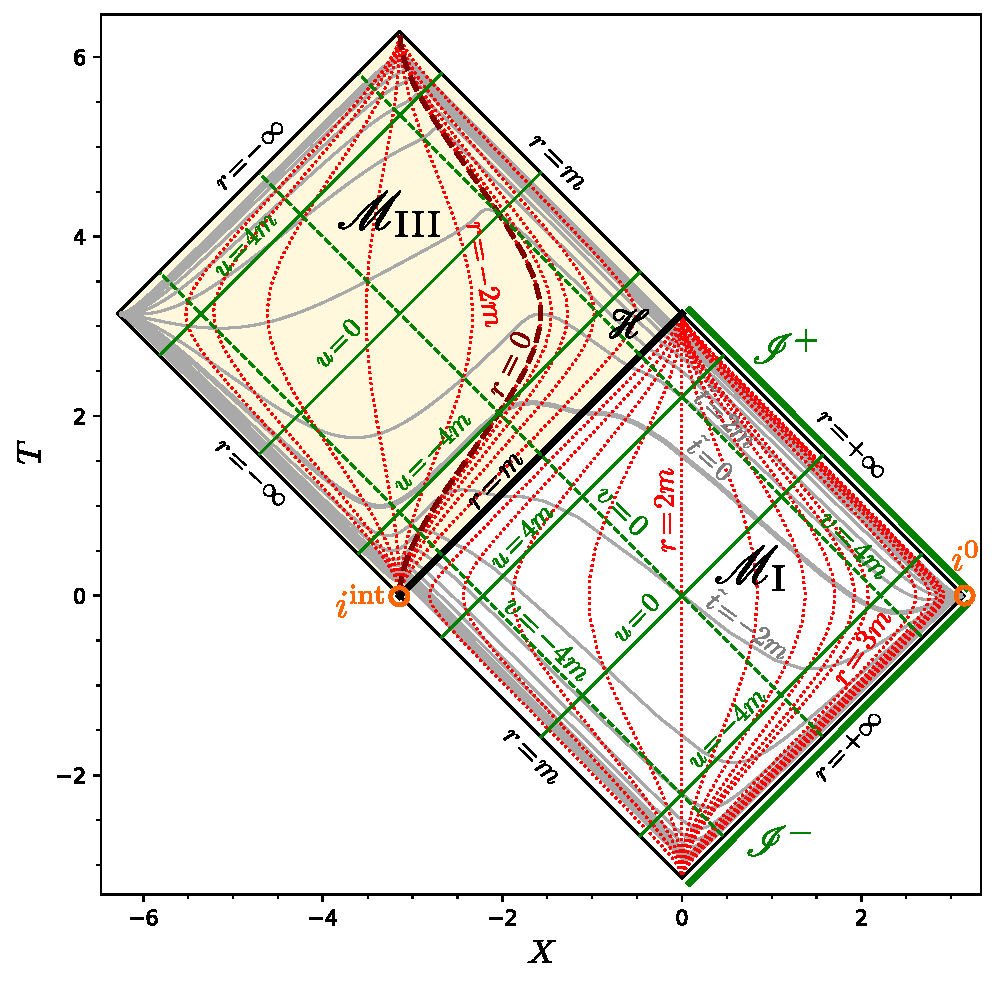
\includegraphics[width=0.8\textwidth]{exk_CPdiag_Kerr.pdf}}
\caption[]{\label{f:exk:CPdiag_Kerr} \footnotesize
Carter-Penrose diagram of the extremal Kerr spacetime $(\M,\w{g})$
constructed via the projection
map $\Pi:\ \M \to \R^2$,  $(\ti,r,\th,\tph)\mapsto (T, X)$
defined by Eqs.~(\ref{e:exk:projection_M})-(\ref{e:exk:def_T0_X0}).
The grey curves represent hypersurfaces $\ti=\mathrm{const}$, with
$\ti\in[-20 m, 20 m]$ and
the increment $\delta\ti = 2 m$ between two successive hypersurfaces.
The hypersurface $\ti=0$ is singled out by a larger thickness.
The red dotted curves represent hypersurfaces $r=\mathrm{const}$,
with the increment $\delta r$ between two successive hypersurfaces being
$\delta r = 2m$ for $r<0$ and $r> 3m$ and $\delta r = 0.2\, m$ for $0\leq r \leq 3m$.
The hypersurface $r=0$ is marked by the brown dashed curve.
The green straight lines depict some selected principal null geodesics
(dashed = ingoing, solid = outgoing, as in Fig.~\ref{f:exk:princ_null_geod}).
\textsl{[Figure generated by the notebook \ref{s:sam:Kerr_extremal}]}
}
\end{figure}


\begin{figure}
\centerline{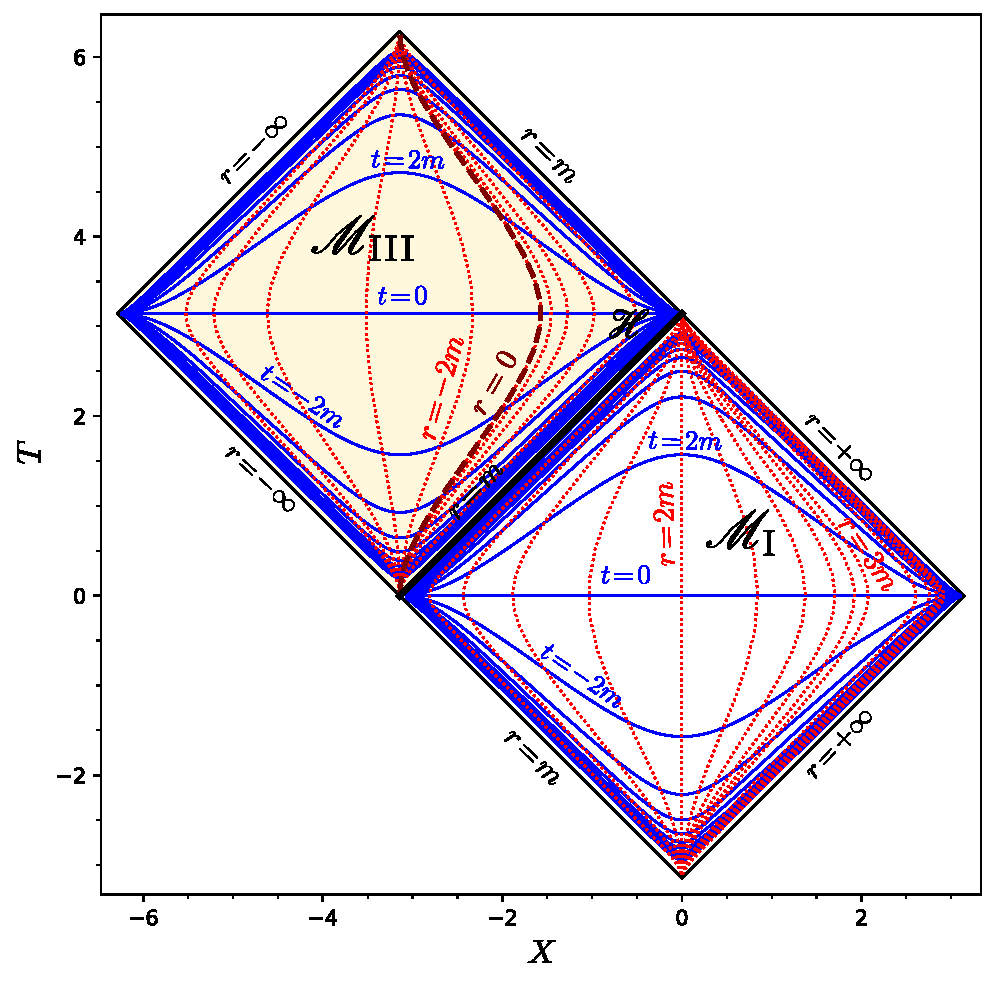
\includegraphics[width=0.8\textwidth]{exk_CPdiag_BL.pdf}}
\caption[]{\label{f:exk:CPdiag_BL} \footnotesize
Same as Fig.~\ref{f:exk:CPdiag_Kerr} but for the
time slicing associated to Boyer-Lindquist coordinates $(t,r,\th,\ph)$.
The blue curves represent hypersurfaces $t=\mathrm{const}$, with
$t\in[-20 m, 20 m]$ and
the increment $\delta t = 2 m$ between two successive hypersurfaces.
Note that the spacetime slicing by the hypersurfaces $t=\mathrm{const}$
is singular at $\Hor$, contrary to the slicing by the hypersurfaces
of constant Kerr time $\ti$ shown in Fig.~\ref{f:exk:CPdiag_Kerr}.
\textsl{[Figure generated by the notebook \ref{s:sam:Kerr_extremal}]}
}
\end{figure}

%%%%%%%%%%%%%%%%%%%%%%%%%%%%%%%%%%%%%%%%%%%%%%%%%%%%%%%%%%%%%%%%%%%%%%%%%%%%%%%

\section{Maximal analytic extension}

\subsection{Extension of $\M_{\rm I}$ for complete outgoing principal null geodesics}

Figure~\ref{f:exk:CPdiag_Kerr} depicts a Carter-Penrose diagram of
the extremal Kerr spacetime $(\M,\w{g})$ built by means of the projection
map\footnote{cf. the definition of a Carter-Penrose diagram given in
Sec.~\ref{s:ker:Carter_Penrose_diag}.}
$\Pi: \M \to \R^2, (\ti, r, \th,\tph) \mapsto (T,X)$ defined by
\begin{subequations}
\label{e:exk:projection_M}
\begin{align}
   & T = T_0(u, v) \qand X = X_0(u, v) \quad\mbox{in}\ \M_{\rm I} \\
   & T = \arctan(v/2) + \pi/2 \qand X = \arctan(v/2) - \pi/2 \quad\mbox{on} \ \Hor \\
   & T = T_0(u, v) + \pi \qand X = X_0(u, v) - \pi \quad\mbox{in}\ \M_{\rm III}
\end{align}
\end{subequations}
with
\begin{subequations}
\label{e:exk:def_T0_X0}
\begin{align}
 & T_0(u, v) := \arctan\left(\frac{u}{2}\right) + \arctan\left(\frac{v}{2}\right) \\
 & X_0(u, v) := \arctan\left(\frac{v}{2}\right)  - \arctan\left(\frac{u}{2}\right) ,
\end{align}
\end{subequations}
where $u$ and $v$ are the functions of $(\ti, r)$ given by
Eqs.~(\ref{e:exk:def_u}) and (\ref{e:exk:def_v}) respectively.
Some outgoing principal null geodesics
$\Li^{\rm out, I}_{(u,\th,\tilde{\tph})}$ and $\Li^{\rm out, III}_{(u,\th,\tilde{\tph})}$
are plotted in Fig.~\ref{f:exk:CPdiag_Kerr}
for selected values of $u$ (solid green lines): $u=-4m$, $u=0$ and $u=4m$.
Since $r$ is an affine parameter along the null geodesics $\Li^{\rm out, I}_{(u,\th,\tilde{\tph})}$,
it is clear that these geodesics are incomplete, for they all terminate
in the past at the finite value $r=m$ (the South-West boundary
of $\M_{\rm I}$ in Fig.~\ref{f:exk:CPdiag_Kerr}), without any possible
extension into $\M_{\rm III}$ from there.
To extend $\M_{\rm I}$ so that all geodesics $\Li^{\rm out, I}_{(u,\th,\tilde{\tph})}$
are complete, let us introduce a coordinate system on $\M_{\rm I}$ that is
adapted to the outgoing principal null geodesics, as the Kerr coordinates
$(\ti,r,\th,\tph)$ were adapted to the ingoing ones.
We thus define the \defin{outgoing Kerr coordinates}\index{outgoing!Kerr coordinates}\index{Kerr!coordinates!outgoing --} $(x^{\tilde{\tilde\alpha}})=(\tilde{\ti},r,\th,\tilde{\tph})$ by
\be \label{e:exk:ttt_u}
    u = \tilde{\ti} - r \iff \tilde{\ti} = u + r  ,
\ee
where $u$ is the retarded Kerr time (\ref{e:exk:def_u}) and $\tilde{\tph}$
is related to the angle $\tph$ of Kerr coordinates or to the angle
$\ph$ of Boyer-Lindquist coordinates by Eq.~(\ref{e:exk:def_ttph}).
Substituting Eq.~(\ref{e:exk:def_u}) for $u$ into $\tilde{\ti} = u + r$
and using Eq.~(\ref{e:exk:def_ttph}) linking $\tilde{\tph}$ to $\tph$,
we get the transition map between the Kerr coordinates $(\ti,r,\th,\tph)$
and the outgoing Kerr coordinates $(\tilde{\ti},r,\th,\tilde{\tph})$:
\be \label{e:exk:Kerr_to_out_Kerr}
    \mbox{on}\, \M_{\rm I},\quad  \left\{
    \begin{array}{l}
    \displaystyle \tilde{\ti}  = \ti + \frac{4 m^2}{r - m}
                        - 4 m \ln \left( \frac{r - m}{m} \right) \\[2ex]
    \displaystyle \tilde{\tph}  = \tph + \frac{2m}{r -m} .
    \end{array} \right.
\ee


By construction, the tangent vector to $\Li^{\rm out, I}_{(u,\th,\tilde{\tph})}$
associated with the affine parameter $r$ is then
\be \label{e:exk:def_ell_prime}
    \wl' = \wpar_{\tilde{\ti}} + \wpar_{\tilde{\tilde{r}}},
\ee
where $\wpar_{\tilde{\tilde{r}}}$ stands for the vector $\partial/\partial r$
of the coordinates $(\tilde{\ti},r,\th,\tilde{\tph})$.
Indeed ${\ell'}^{\tilde{\tilde\alpha}} = \D x^{\tilde{\tilde\alpha}} /\D r
= (1, 1, 0, 0)$ since along $\Li^{\rm out, I}_{(u,\th,\tilde{\tph})}$,
$\tilde{\ti} = r + u$, with $u$ constant, and both $\th$ and $\tilde{\tph}$
are constant. An explicit computation (cf. the notebook~\ref{s:sam:Kerr_extremal_extended}) shows that
$\wl'$ is a geodesic vector:
\be
    \wnab_{\wl'} \wl' = 0 ,
\ee
which confirms that $r$ is an affine parameter along $\Li^{\rm out, I}_{(u,\th,\tilde{\tph})}$.
$\wl'$ is thus similar to $\w{k}$, which is
the tangent vector to the \emph{ingoing} principal null geodesics $\Li^{\rm in}_{(v,\th,\tph)}$
associated with the affine parameter $-r$ along them.
In this respect, note the symmetry between the relations
$\wl' = \wpar_{\tilde{\ti}} + \wpar_{\tilde{\tilde{r}}}$
and $\w{k} = \wpar_{\ti} - \wpar_{\tilde{r}}$ [Eq.~(\ref{e:exk:k_3p1_Kerr})].
The link between $\wl'$ and the tangent vector $\wl$ to $\Li^{\rm out, I}_{(u,\th,\tilde{\tph})}$
introduced in Sec.~\ref{s:exk:princ_null_geod} is easily obtained from
the definition of a tangent vector to a curve:
\[
    \wl' = \frac{\D\w{x}}{\D r} = \frac{\D\w{x}}{\D\lambda} \frac{\D\lambda}{\D r}
        = \left(\frac{\D r}{\D \lambda} \right) ^{-1} \wl ,
\]
where $\lambda$ is the (non-affine) parameter of $\Li^{\rm out, I}_{(u,\th,\tilde{\tph})}$
associated with $\wl$. We read on the Kerr components (\ref{e:exk:ell_3p1_Kerr})
of $\wl$, as well as on the Boyer-Lindquist ones (\ref{e:exk:ell_BL}), that
$\D r/\D\lambda = \ell^r = (r-m)^2/(2(r^2 + m^2))$. Hence
\be \label{e:exk:ell_prime_ell}
    \wl' = 2 \frac{r^2 + m^2}{(r - m)^2} \, \wl .
\ee

Differentiating Eq.~(\ref{e:exk:Kerr_to_out_Kerr})
leads to
\be \label{e:exk:Dttt_Dtph_Kerr}
    \D\tilde{\ti} = \D\ti - \frac{4 m r}{(r-m)^2} \D r
    \qand
    \D\tilde{\tph} = \D\tph - \frac{2 m}{(r-m)^2} \D r .
\ee
From these relations and the chain rule, we get immediately
the link between the outgoing Kerr coordinate frame and the Kerr coordinate frame:
\be \label{e:exk:out_Kerr_frame}
    \wpar_{\tilde{\ti}} = \wpar_{\ti},\qquad
    \wpar_{\tilde{\tilde{r}}} = \wpar_{\tilde{r}} + \frac{4 m r}{(r-m)^2} \wpar_{\ti}
        + \frac{2m}{(r-m)^2} \wpar_{\tph}, \qquad
    \wpar_{\th} = \wpar_{\th},\qquad
    \wpar_{\tilde{\tph}} = \wpar_{\tph} .
\ee
In view of Eq.~(\ref{e:exk:Killing_vectors}), we conclude that
$\wpar_{\tilde{\ti}}$ and $\wpar_{\tilde{\tph}}$ coincide
with the Killing vectors $\w{\xi}$ and $\w{\eta}$ of the Kerr metric:
\be
    \wpar_{\tilde{\ti}} = \w{\xi} \qand \wpar_{\tilde{\tph}} = \w{\eta} .
\ee

The link between the outgoing Kerr coordinates and the Boyer-Lindquist ones
is obtained by substituting Eq.~(\ref{e:exk:def_u}) for $u$ into $\tilde{\ti} = u + r$
[Eq.~(\ref{e:exk:ttt_u})]:
\be \label{e:exk:ttt_t}
    \tilde{\ti} = t + \frac{2m^2}{r -m} - 2m\ln\left| \frac{r - m}{m} \right| .
\ee
This relation is to be supplemented by Eq.~(\ref{e:exk:def_ttph}) to fully
specify the transformation from the Boyer-Lindquist coordinates
$(t,r,\th,\ph)$ to the outgoing Kerr coordinates
$(\tilde{\ti},r,\th,\tilde{\tph})$.
Differentiating Eqs.~(\ref{e:exk:ttt_t}) and (\ref{e:exk:def_ttph})
leads to
\be \label{e:exk:Dttt_Dtph_BL}
    \D\tilde{\ti} = \D t - \frac{2 m r}{(r-m)^2} \D r
    \qand
    \D\tilde{\tph} = \D\ph - \frac{m}{(r-m)^2} \D r
\ee
\begin{remark}
Equation~(\ref{e:exk:Dttt_Dtph_BL}) differs from
Eq.~(\ref{e:exk:dt_dph}) only by the sign $+$ changed to $-$ in the
right-hand side. This reflects the complete symmetry between the Kerr coordinates
$(\ti,r,\th,\tph)$
and the outgoing Kerr coordinates
$(\tilde{\ti},r,\th,\tilde{\tph})$
from the point of view of the Boyer-Lindquist coordinates $(t,r,\th,\ph)$
(cf. the discussion at the beginning of Sec.~\ref{s:ker:out_princ_null_geod}).
\end{remark}


The components of the metric tensor $\w{g}$ with respect to the
outgoing Kerr coordinates are easily obtained by substituting $\D t$ and $\D\ph$
from Eq.~(\ref{e:exk:Dttt_Dtph_BL}) into the Boyer-Lindquist expression
(\ref{e:exk:metric_BL}) (see also the notebook~\ref{s:sam:Kerr_extremal_extended}); we get
\be \label{e:exk:metric_out_Kerr}
    \begin{array}{ll}
    g_{\tilde{\tilde{\mu}}\tilde{\tilde{\nu}}}\, \D x^{\tilde{\tilde{\mu}}} \, \D x^{\tilde{\tilde{\nu}}}   = &
    \displaystyle - \left( 1 - \frac{2m r}{\rho^2} \right)  {\D\tilde{\ti}}^2
    - \frac{4m r}{\rho^2} \D\tilde{\ti}\, \D r
    - \frac{4 m^2  r \sin^2\th}{\rho^2} \,  \D\tilde{\ti}\, \D\tilde{\tph} \\[2ex]
    &\displaystyle  + \left( 1 + \frac{2m r}{\rho^2} \right) \D r^2
     + 2 m \left( 1 + \frac{2m r}{\rho^2} \right) \sin^2\th \, \D r\, \D\tilde{\tph} \\[2ex]
    & \displaystyle + \rho^2 \D \th^2
    + \left( r^2 + m^2 + \frac{2 m^3 r \sin^2\th}{\rho^2} \right)
    \sin^2\th \, {\D\tilde{\tph}}^2 .
    \end{array}
\ee
These metric components are very similar to those in Kerr coordinates, as given by
Eq.~(\ref{e:exk:metric_Kerr_3p1}): the only differences are $g_{\tilde{\ti}r}$ and
$g_{r\tilde{\tph}}$, which have a sign opposite to that of respectively $g_{\ti r}$
and $g_{r\tph}$. Apart from the standard singularities of the
spherical coordinates $(\th,\tilde{\tph})$ on the axis $\th\in\{0,\pi\}$, the
only singularity of the metric components (\ref{e:exk:metric_out_Kerr})
would occur at $\rho=0$, which does not happen in $\M_{\rm I}$. In particular
there is no divergence for $r\to m$. This can be used to extend smoothly
the spacetime $(\M_{\rm I},\w{g})$ to $r\in(-\infty, m]$, so that the outgoing
principal null geodesics $\Li^{\rm out, I}_{(u,\th,\tilde{\tph})}$
with $\th\neq \pi/2$ become
complete. But the extension to $r<m$ cannot be $\M_{\rm III}$
as it appears clearly on Fig.~\ref{f:exk:CPdiag_Kerr} that  the end point
of $\Li^{\rm out, I}_{(u,\th,\tilde{\tph})}$ for $r\to m^+$ is not located at the
boundary between $\M_{\rm I}$ and $\M_{\rm III}$.
We thus introduce a spacetime $(\M',\w{g})$ from a new copy of
$\R^2\times\SS^2$ with $\R^2$ spanned by the coordinates $(\tilde{\ti},r)$ and
$\SS^2$ spanned by the coordinates $(\th,\tilde{\tph})$, such that (i)
the manifold $\M'$ is
\be
 \M' := \R^2\times\SS^2 \setminus \ring'
 \quad\mbox{where}\quad
    \ring' := \left\{ p \in \R^2\times\SS^2,
        \quad r(p) = 0 \ \mbox{and}\ \th(p) = \frac{\pi}{2} \right\} ,
\ee
(ii) $\M_{\rm I}$ is identified with the part $r>m$ of $\M'$ and
(iii) in all $\M'$, $\w{g}$ has the components given by expression
(\ref{e:exk:metric_out_Kerr}). Furthermore, we define
\be
    \Hor' := \left\{ p \in \M', \quad r(p) = m \right\}
    \qand
    {\M'}_{\rm III} := \left\{ p \in \M', \quad r(p) < m \right\} .
\ee
We have then $\M_{\rm I} = \M \cap \M'$.
In ${\M'}_{\rm III}$, one can define Kerr coordinates $(\ti,r,\th,\tph)$
from $(\tilde{\ti},r,\ph,\tilde{\tph})$
via formulas (\ref{e:exk:def_u}) (with $u = \tilde{\ti} - r$) and (\ref{e:exk:def_ttph}).
It appears then immediately that $({\M'}_{\rm III}, \w{g})$ is isometric to $(\M_{\rm III},\w{g})$.
It follows that $\w{g}$ obeys the vacuum Einstein equation in all $\M'$.
The vector field $\wl' := \wpar_{\tilde{\ti}} + \wpar_{\tilde{\tilde{r}}}$
[cf. Eq.~(\ref{e:exk:def_ell_prime})] is a smooth non-vanishing null vector
field on $\M'$. Since it is future directed in $(\M_{\rm I},\w{g})$
considered as a part of $(\M,\w{g})$,
we use it to set the time orientation in all $\M'$.

The tangent vector $\w{k}$ to ingoing principal null geodesics has
the following components with respect to the outgoing Kerr coordinates:
\be \label{e:exk:k_out_Kerr}
    \w{k} = \frac{(r + m)^2}{(r - m)^2} \, \wpar_{\tilde{\ti}}
    - \wpar_{\tilde{\tilde{r}}} + \frac{2m}{(r - m)^2} \, \wpar_{\tilde{\tph}} .
\ee
This follows immediately from
$\w{k} = \wpar_{\ti} - \wpar_{\tilde{r}}$ [Eq.~(\ref{e:exk:k_3p1_Kerr})]
and using Eq.~(\ref{e:exk:out_Kerr_frame})
to substitute $\wpar_{\ti}$ and $\wpar_{\tilde{r}}$.
Extending Equation~(\ref{e:exk:k_out_Kerr}) to all $\M'$
leads to a vector field that is singular on $\Hor'$. To get a vector field
everywhere regular on $\M'$, we rescale it by the inverse of the factor
relating $\wl$ to $\wl'$ in Eq.~(\ref{e:exk:ell_prime_ell}), i.e. we
define
\be
    \w{k}' := \frac{(r - m)^2}{2(r^2 + m^2)} \, \w{k} .
\ee
Hence
\be \label{e:exk:k_prime_out_Kerr}
    \w{k}' = \frac{(r + m)^2}{2(r^2 + m^2)} \, \wpar_{\tilde{\ti}}
    - \frac{(r-m)^2}{2(r^2 + m^2)}\, \wpar_{\tilde{\tilde{r}}} + \frac{m}{r^2 + m^2} \, \wpar_{\tilde{\tph}} .
\ee
This vector field is clearly regular in all $\M'$.
Accordingly, it can be used to extend smoothly the family of ingoing principal
null geodesics to $\Hor'$. The price to pay is that $\w{k}'$ is only a pregeodesic
vector field, while $\w{k}$ was geodesic, being associated with the affine parameter $-r$.
The pair $(\w{k}, \w{k}')$ plays actually the same role as the pair $(\wl', \wl)$
(note the order!) regarding the outgoing principal null geodesics.

\begin{figure}
\centerline{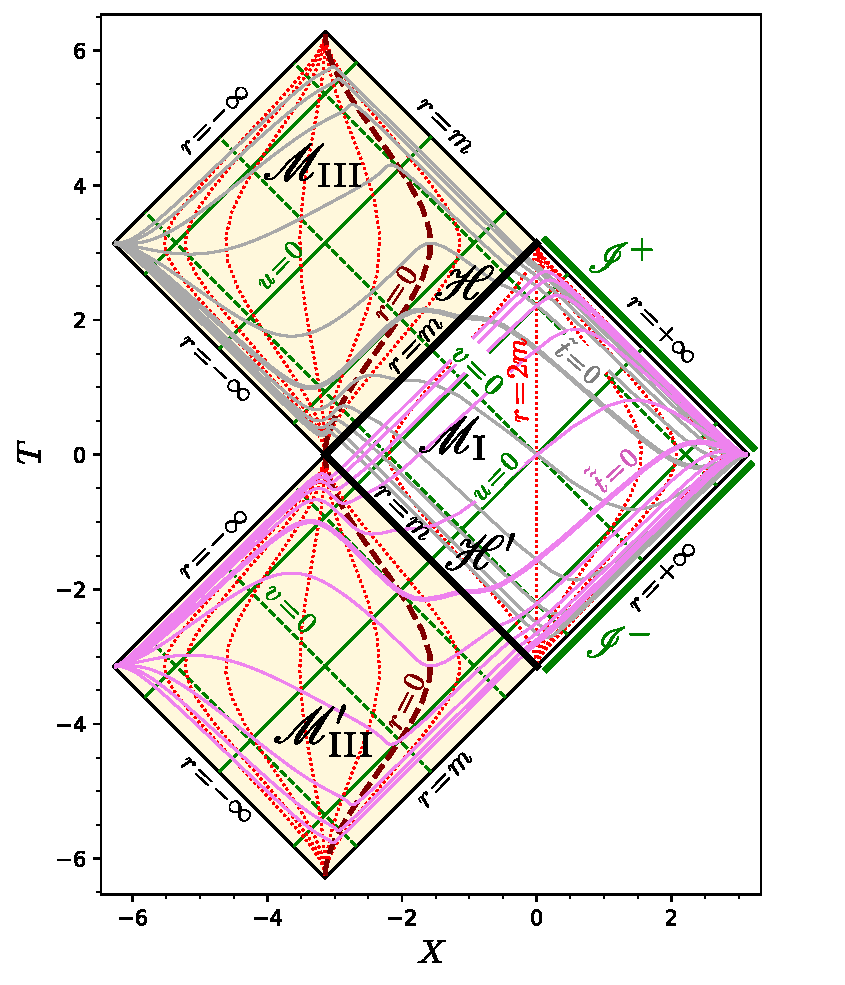
\includegraphics[width=0.8\textwidth]{exk_CPdiag_M0.pdf}}
\caption[]{\label{f:exk:CPdiag_M0} \footnotesize
Carter-Penrose diagram of the (partially) extended extremal Kerr spacetime $(\M_0,\w{g})$.
The grey curves represent hypersurfaces $\ti=\mathrm{const}$ in $\M$, with
$\ti\in[-10 m, 10 m]$ and
the increment $\delta\ti = 2 m$ between two successive hypersurfaces.
The hypersurface $\ti=0$ is singled out by a larger thickness.
The purple curves represent hypersurfaces $\tilde{\ti}=\mathrm{const}$ in $\M'$, with
$\tilde{\ti}\in[-10 m, 10 m]$ and
the increment $\delta\tilde{\ti} = 2 m$ between two successive hypersurfaces.
The hypersurface $\tilde{\ti}=0$ is singled out by a larger thickness.
The red dotted curves represent hypersurfaces $r=\mathrm{const}$,
with the increment $\delta r$ between two successive hypersurfaces being
$\delta r = 2m$ for $r<0$ and $r> 3m$ and $\delta r = 0.5\, m$ for $0\leq r \leq 3m$.
The hypersurfaces $r=0$ are marked by brown dashed curves.
The dashed (resp. solid) green straight lines depict some selected ingoing (resp. outgoing)
principal null geodesics.
\textsl{[Figure generated by the notebook \ref{s:sam:Kerr_extremal_extended}]}
}
\end{figure}

As $\Hor$ in $(\M,\w{g})$, $\Hor'$ is a degenerate Killing horizon of $(\M',\w{g})$.
Indeed, by the same reasoning as in Sec.~\ref{s:exk:horizon}, we get that
the null normal to $\Hor'$ is the Killing vector
$\w{\chi} = \w{\xi} + 1/(2m) \, \w{\eta}$ [Eq.~(\ref{e:exk:def_chi}) extended to
$\M'$]. This normal coincides with $\w{k}'$ on $\Hor'$, as we can see
by setting $r=m$ in  Eq.~(\ref{e:exk:k_prime_out_Kerr}). This implies that
the null geodesic generators of  $\Hor'$ belong to the ingoing principal null congruence.
The non-affinity coefficient of $\w{k}'$ is (cf. the notebook~\ref{s:sam:Kerr_extremal_extended}):
\be
    \kappa_{\w{k}'} = m \frac{m^2 - r^2}{(r^2 + m^2)^2} .
\ee
We have thus $\kappa_{\w{k}'} = 0$ on $\Hor'$, so that $\Hor'$ is a
degenerate Killing horizon.

With $\M'$, our extended extremal Kerr spacetime is thus $(\M_0,\w{g})$ with
\be
   \encadre{ \M_0 := \M \cup \M'
     = \M_{\rm I} \cup \M_{\rm III} \cup \M'_{\rm III} \cup \Hor \cup \Hor' } .
\ee
A Carter-Penrose diagram of $\M_0$ is shown in Fig.~\ref{f:exk:CPdiag_M0}.
The projection operator used to build this diagram (cf. Sec.~\ref{s:ker:Carter_Penrose_diag})
is $\Pi : \M_0 \to \R^2$, with $\R^2$ spanned by coordinates $(T,X)$,
such that $\Pi$ is defined by Eqs.~(\ref{e:exk:projection_M})-(\ref{e:exk:def_T0_X0})
on $\M$, while on $\M'$, $\Pi$ is defined by
\begin{subequations}
\begin{align}
   & T = T_0(u, v) \qand X = X_0(u, v) \quad\mbox{in}\ \M_{\rm I} \\
   & T = \arctan(u/2) - \pi/2 \qand X = -\arctan(u/2) - \pi/2 \quad\mbox{on} \ \Hor' \\
   & T = T_0(u, v) - \pi \qand X = X_0(u, v) - \pi \quad\mbox{in}\ \M'_{\rm III}
\end{align}
\end{subequations}
where $T_0(u,v)$ and $X_0(u,v)$ are given by Eq.~(\ref{e:exk:def_T0_X0})
and $u$ and $v$ are functions of $(\tilde{\ti}, r)$ defined by
respectively $u = \tilde{\ti} - r$ [Eq.~(\ref{e:exk:ttt_u})]
and
\be
    v = \tilde{\ti} + r - \frac{4 m^2}{r - m} + 4 m \ln \left| \frac{r - m}{m} \right| .
\ee
The last equation is obtained by combining Eqs.~(\ref{e:exk:def_v}) and (\ref{e:exk:def_u}).


\begin{remark}
As we have constructed it, the manifold $\M_0$ is covered by two coordinate charts:
$(\ti, r, \th, \tph)$ on $\M_{\rm I} \cup \Hor \cup \M_{\rm III}$
and $(\tilde{\ti}, r, \th, \tilde{\tph})$ on $\M_{\rm I} \cup \Hor' \cup \M'_{\rm III}$.
These two charts overlap in $\M_{\rm I}$, where the transition between them
is provided by Eq.~(\ref{e:exk:Kerr_to_out_Kerr}).
The Carter-Penrose diagram of Fig.~\ref{f:exk:CPdiag_M0} might give the impression
that, by means of the coordinates $(T,X)$, one could cover $\M_0$ by a single chart,
in a fashion similar to the covering of the entire maximal extension of Schwarzschild
spacetime by the Kruskal-Szekeres coordinates\index{Kruskal-Szekeres!coordinates}
$(T,X,\th,\ph)$ (cf. Sec.~\ref{s:sch:max_extens}). However, this is not possible
in a simple way, due to singularity issues with the azimuthal coordinates:
$\tph$ diverges on $\Hor'$, $\tilde{\tph}$ diverges on $\Hor$ and
the Boyer-Lindquist coordinate $\ph$ diverges on both $\Hor$ and $\Hor'$.
Accordingly, none of $(T,X,\th,\tph)$, $(T,X,\th,\tilde{\tph})$ and
$(T,X,\th,\ph)$ would provide a regular chart of $\M_0$.
\end{remark}

\begin{remark} \label{r:exk:M0_analytic}
The spacetime $(\M_0,\w{g})$ is analytic: (i) $\M_0$ is an analytic manifold,
given that the change of coordinates (\ref{e:exk:Kerr_to_out_Kerr})
between the two charts covering $\M_0$ is analytic
(cf. Remark~\ref{r:bas:analytic} in Sec.~\ref{s:bas:def_manif})
and (ii) the components (\ref{e:exk:metric_Kerr_3p1}) and (\ref{e:exk:metric_out_Kerr})
of $\w{g}$ are analytic functions of the
coordinates $(\ti, r, \th, \tph)$ and $(\tilde{\ti}, r, \th, \tilde{\tph})$
respectively.
\end{remark}


The Killing horizon $\Hor'$ is actually a white hole horizon from the point
of view of $\M_{\rm I}$. More precisely, we can endow $(\M_0,\w{g})$ with the same conformal
completion at null infinity as that used for $(\M,\w{g})$ in Sec.~\ref{s:exk:bhole_char},
i.e. such that the conformal boundary $\scri$ is constituted by
the same future and past null infinities
$\scri^+$ and $\scri^-$ located at the boundary of $\M_{\rm I}$ (cf. Fig.~\ref{f:exk:CPdiag_M0}).
It appears then that
\be
   \M'_{\rm III}\cup \Hor' = \M_0 \setminus (J^+(\scri^-)\cap \M_0)
\ee
In view of the definition (\ref{e:glo:def_white_hole}), we conclude that
\begin{greybox}
$\M'_{\rm III}$ is the interior of a white hole\index{white hole} region, the boundary of which
is $\Hor'$.
\end{greybox}

Since $\M_{\rm III}$ was shown in Sec.~\ref{s:exk:bhole_char} to be the black hole region for
the same conformal completion at null infinity, we may state,
according to the terminology introduced in Sec.~\ref{s:glo:def_BH}:
\begin{greybox}
$\M_{\rm I}$ is the domain of outer communications\index{domain!of outer communications}
of the spacetime $(\M_0,\w{g})$.
\end{greybox}


\begin{figure}
\centerline{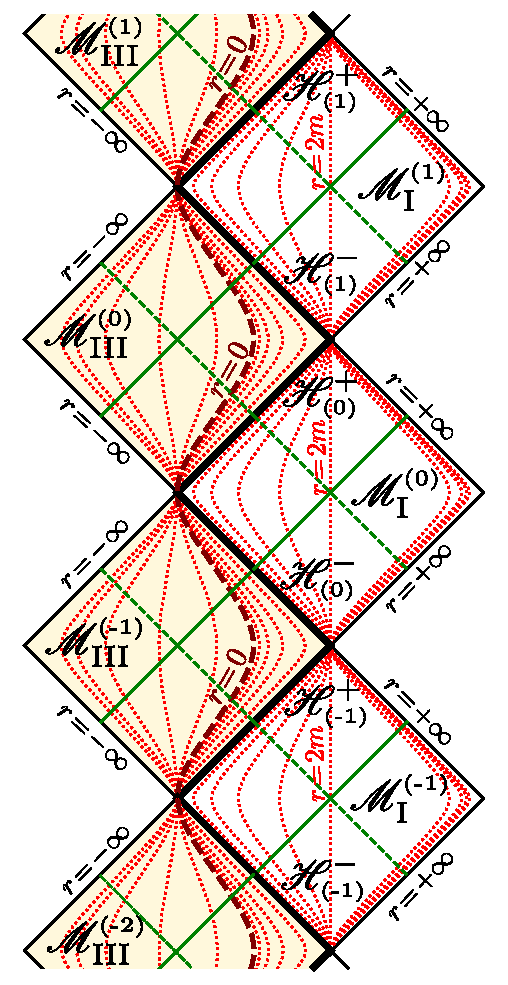
\includegraphics[height=0.7\textheight]{exk_CPdiag_maximal.pdf}}
\caption[]{\label{f:exk:CPdiag_maximal} \footnotesize
Carter-Penrose diagram of the maximal analytic extension $(\M_*,\w{g})$
of the extremal Kerr spacetime.
The red dotted curves represent hypersurfaces $r=\mathrm{const}$,
with the increment $\delta r$ between two successive hypersurfaces being
$\delta r = 2m$ for $r<0$ and $r> 2m$ and $\delta r = 0.2\, m$ for $0\leq r \leq 2m$.
The hypersurfaces $r=0$ are marked by brown dashed curves.
The dashed (resp. solid) green straight lines depict ingoing (resp. outgoing)
principal null geodesics with $v=0$ (resp. $u=0$).
\textsl{[Figure generated by the notebook \ref{s:sam:Kerr_extremal_extended}]}
}
\end{figure}

\subsection{Construction of the maximal analytic extension}

With $(\M_0,\w{g})$, we have acheived our first goal: all the outgoing
principal null geodesics crossing $\M_{\rm I}$ and not lying in the equatorial
plane (i.e. the geodesics extending the $\Li^{\rm out, I}_{(u,\th,\tilde{\tph})}$
family with $\th\neq \pi/2$ to the past) are complete. However, there remains
incomplete geodesics in $\M_0$: the outgoing principal null geodesics crossing $\M_{\rm III}$
all stop at the value $r=m$ of their affine parameter, while
the ingoing principal null geodesics crossing $\M'_{\rm III}$ all start at the
value $-r = -m$ of their affine parameter (cf. Fig.~\ref{f:exk:CPdiag_M0}).
To construct a spacetime with complete geodesics, except for those that encouter the curvature singularity at $r=0$ and $\th=\pi/2$, one introduces an infinite number of copies of $\M_0$,
$\left( \M_n \right)_{n\in\mathbb{Z}}$ say, and identify the region $\M'_{\rm III}$ of $\M_n$
with the region $\M_{\rm III}$ of $\M_{n-1}$ for all $n\in\mathbb{Z}$.
The manifold hence obtained,
\be
    \M_* := \bigcup_{n\in\mathbb{Z}} \M_n ,
\ee
is depicted via a
Carter-Penrose diagram in Fig.~\ref{f:exk:CPdiag_maximal}.
The region $\M_{\rm I}$ (resp. $\M_{\rm III}$) of $\M_n$ is
denoted by $\M_{\rm I}^{(n)}$ (resp. $\M_{\rm III}^{(n)}$). Similarly,
the Killing horizon $\Hor$ (resp. $\Hor'$) of $\M_n$ is denoted
by $\Hor_{(n)}^+$ (resp. $\Hor_{(n)}^-$). Note that $\Hor_{(n)}^+$
is a future event horizon (black hole horizon), while
$\Hor_{(n)}^-$ is a past event horizon (white hole horizon),
for the conformal completion at null infinity with
the future and past null infinities $\scri^+_{(n)}$ and $\scri^-_{(n)}$
as copies of $\scri^+$ and $\scri^-$ introduced for $\M_0$.

It is clear that $(\M_*,\w{g})$ is an analytic spacetime, since $(\M_0,\w{g})$
is (cf. Remark~\ref{r:exk:M0_analytic} on p.~\pageref{r:exk:M0_analytic}).

By construction, all principal null geodesics are complete in $\M_*$,
except for those that encounter the curvature singularity at
$r=0$ and $\th=\pi/2$. In particular, this holds for the outgoing
principal null geodesics generating $\Hor_{(n)}^+$
and for the ingoing ones generating $\Hor_{(n)}^-$.
Contemplating the Carter-Penrose diagram of Fig.~\ref{f:exk:CPdiag_maximal},
we might thus perceive each (solid or dashed) green straight line
from an $r=-\infty$ end to an $r=+\infty$ end, as well as
each thick black straight line, as representating a complete principal null
geodesic.

It can be shown that actually \emph{all} timelike or null
geodesics of $(\M_*,\w{g})$, and not only the principal null ones, are complete
(see Carter's article \cite{Carte68a} for the proof), so that we can conclude:
\begin{greybox}
$(\M_*,\w{g})$ is the maximal analytic extension of the
extremal Kerr spacetime.
\end{greybox}

\begin{remark}
The construction of the maximal extension of the extremal Kerr spacetime
is simpler than that of the Kerr spacetime with $a<m$, as presented
in Sec.~\ref{s:ker:max_extension}. Indeed, for the latter, if one uses
only the ingoing and outgoing Kerr coordinate patches $(\ti,r,\th,\tph)$
and $(\tilde{\ti},r,\th,\tilde{\tph})$, one ends up with a manifold that
is not maximal: the null geodesics generating the Killing horizons
at $r=r_\pm$ are not complete, because the bifurcation spheres\index{bifurcation!sphere}
(the central dots in Fig.~\ref{f:ker:max_ext}), accross which these geodesics
can be extended, are missing.
Indeed the bifurcation spheres are not covered by Kerr coordinates.
To include them and thus get the full bifurcate Killing horizons
(cf. Sec.~\ref{s:sta:bifur_Killing_hor}), one has to introduce Kruskal-Szekeres-type
coordinates in the vicinity of each bifurcation sphere, in a way similar to
the Schwarzschild case treated in Secs.~\ref{s:max:KS} and \ref{s:sch:max_extens}.
In the present case, each Killing horizon $\Hor^+_{(n)}$ or $\Hor^-_{(n)}$
is degenerate and therefore made of complete null geodesics. In particular,
$\Hor^+_{(n)}$ and $\Hor^-_{(n)}$ are not part of a bifurcate Killing horizon. In other words, there
are no bifurcation spheres in the maximal extension of the extremal Kerr spacetime
and the ingoing and outgoing Kerr coordinate patches
are sufficient to cover it entirely.
\end{remark}

\begin{hist}
In 1966, Brandon Carter\index{Carter, B.} \cite{Carte66} obtained the maximal analytic extension
of the rotation axis $\mathscr{A}$ of the extremal Kerr spacetime (cf. historical note on p.~\pageref{h:ker:max_ext_diag}). In particular, he drew a diagram (Fig.~1b of Ref.~\cite{Carte66})
similar to that of Fig.~\ref{f:exk:CPdiag_maximal}, the difference
being that Carter's one is a true conformal representation, owing to the fact
that $\mathscr{A}$ is 2-dimensional, while the diagram of Fig.~\ref{f:exk:CPdiag_maximal}
is a mere projection of the 4-dimensional manifold $\M_*$.
In their 1967 classical study entitled \emph{Maximal Analytic Extension of the Kerr metric}
\cite{BoyerL67},
Robert H. Boyer\index{Boyer, R.H.} and Richard W. Lindquist\index{Lindquist, R.W.}
focussed on the case $a<m$. For $a=m$, they refered to Carter's study \cite{Carte66}
and stated simply that
\emph{although his
\emph{[Carter's]} work was confined to the symmetry axis ($\th=0,\pi$), it is clear
that his conclusions apply with equal force to the full metric}.
The detailed construction of the maximal analytic extension
of the full extremal Kerr spacetime was actually presented by Carter himself
in 1968 \cite{Carte68a}, as the special case of vanishing electric charge
of the extremal Kerr-Newman spacetime.
The construction was also performed in details in his famous lectures at Les Houches
Summer School in 1972~\cite{Carte73a}.
\end{hist}


%%%%%%%%%%%%%%%%%%%%%%%%%%%%%%%%%%%%%%%%%%%%%%%%%%%%%%%%%%%%%%%%%%%%%%%%%%%%%%%

\section{Near-horizon extremal Kerr metric}

\subsection{The extremal Kerr throat}

Let us consider a hypersurface $\Sigma_t$ of constant Boyer-Lindquist time $t$
in the external region $\M_{\rm I}$ of the extremal Kerr spacetime
(one of the hypersurfaces shown as blue curves in Figs.~\ref{f:exk:BL_slicing}
and \ref{f:exk:CPdiag_BL}).
$\Sigma_t$ is a spacelike hypersurface, since it is clear from
the line element (\ref{e:exk:metric_BL}) that the metric induced by $\w{g}$
on $\Sigma_t$ is Riemannian (i.e. positive definite) in\footnote{The induced
metric would not be Riemannian in the Carter time machine (cf. Sec.~\ref{s:ker:time_machine}),
where $g_{\ph\ph} < 0$;
but this requires $r<0$, while $r>m$ in $\M_{\rm I}$.}
$\M_{\rm I}$.
We may thus vizualise the geometry of $\Sigma_t$ by some isometric embedding
of 2-dimensional slices of $\Sigma_t$ into the Euclidean space $\R^3$,
as we did for the hypersurfaces of constant Kruskal-Szekeres time in
Schwarzschild spacetime in Sec.~\ref{s:max:isometric_emb}. It is then
natural to consider the slices $\Sigma_{t,\th}$ where $\th$ is held constant,
in addition to $t$, with $\Sigma_{t,\frac{\pi}{2}}$ representing the
equatorial ``plane''. $\Sigma_{t,\th}$  is spanned by the coordinates
$(x^a) = (r,\ph)$ and the Riemannian metric $\w{q}$ induced on it by
the spacetime metric $\w{g}$ is obtained by setting $\D t = 0$ and $\D\th = 0$
in the line element (\ref{e:exk:metric_BL}):
\be \label{e:exk:induced_metric_q}
    q_{ab}\,  \D x^a \D x^b  =
    \frac{r^2 + m^2\cos^2\th}{(r-m)^2} \, \D r^2
    + \left( r^2 + m^2 + \frac{2 m^3 r \sin^2\th}{r^2 + m^2\cos^2\th} \right)
    \sin^2\th \, \D \ph^2 .
\ee
Let us consider the Euclidean space $\R^3$ described by
cylindrical coordinates $(X^i) = (\varpi,z,\ph)$. The Euclidean metric $\w{f}$
is then
\be
    f_{ij}\,  \D x^i \D x^j = \D \varpi^2 + \D z^2 + \varpi^2 \D\ph^2 .
\ee
Let us define the embedding of the 2-surface $\Sigma_{t,\th}$ into
$\R^3$ by
\be \label{e:exk:isom_emb_z_r}
    \begin{array}{clcl}
    \Phi: & \Sigma_{t,\th} & \longrightarrow & \R^3 \\
        & (r,\ph) & \longmapsto & (\varpi(r),z(r),\ph) .
    \end{array}
\ee
Along $\Phi(\Sigma_{t,\th})$, we have then
$\D\varpi = \varpi'(r) \, \D r$ and $\D z = z'(r) \, \D r$, so that the
metric $\w{h}$ induced by $\w{f}$ on $\Phi(\Sigma_{t,\th})$ is
\be \label{e:exk:induced_metric_h}
    h_{ab}\,  \D x^a \D x^b  =
    \left( \varpi'(r)^2 + z'(r)^2 \right) \, \D r^2
    + \varpi(r)^2 \, \D\ph^2 .
\ee
$\Phi$ performs an isometric embedding iff the two line elements
(\ref{e:exk:induced_metric_q}) and (\ref{e:exk:induced_metric_h})
coincide\footnote{Formally, one says that the metric $\w{q}$ is the pullback
of $\w{h}$ by $\Phi$: $\w{q} = \Phi^* \w{h}$.}, i.e. iff
\begin{subequations}
\begin{align}
    & \varpi(r) = \sin\th \sqrt{r^2 + m^2 + \frac{2 m^3 r \sin^2\th}{r^2 + m^2\cos^2\th} }
        \label{e:exk:isom_emb_cond1} \\
    &\varpi'(r)^2 + z'(r)^2 = \frac{r^2 + m^2\cos^2\th}{(r-m)^2}  . \label{e:exk:isom_emb_cond2}
\end{align}
\end{subequations}
We deduced from Eq.~(\ref{e:exk:isom_emb_cond2}) that
\be \label{e:exk:isom_emb_z_r}
    z(r) = \int_{2m}^r
    \frac{1}{\bar{r}-m}
    \sqrt{\bar{r}^2 + m^2\cos^2\th
        - \varpi'(\bar{r})^2 (\bar{r}-m)^2 } \; \D \bar{r} ,
\ee
up to some additive constant, which we set to zero by choosing arbitrarily $z(2m) = 0$.
In the integrand, $\varpi'(\bar{r})$ should be substituted by the value obtained
by differentiating Eq.~(\ref{e:exk:isom_emb_cond1}).

\begin{figure}
\centerline{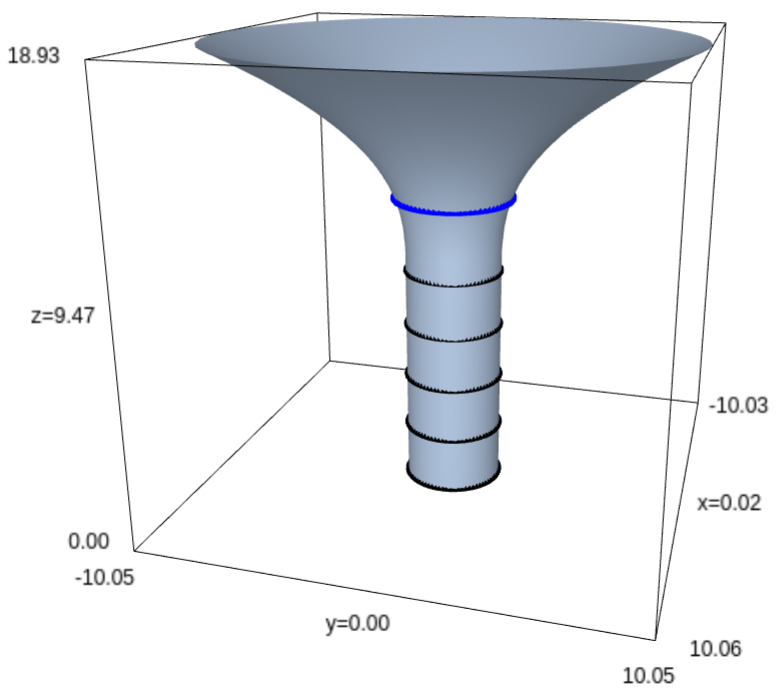
\includegraphics[width=0.6\textwidth]{exk_throat_emb_equat.png}
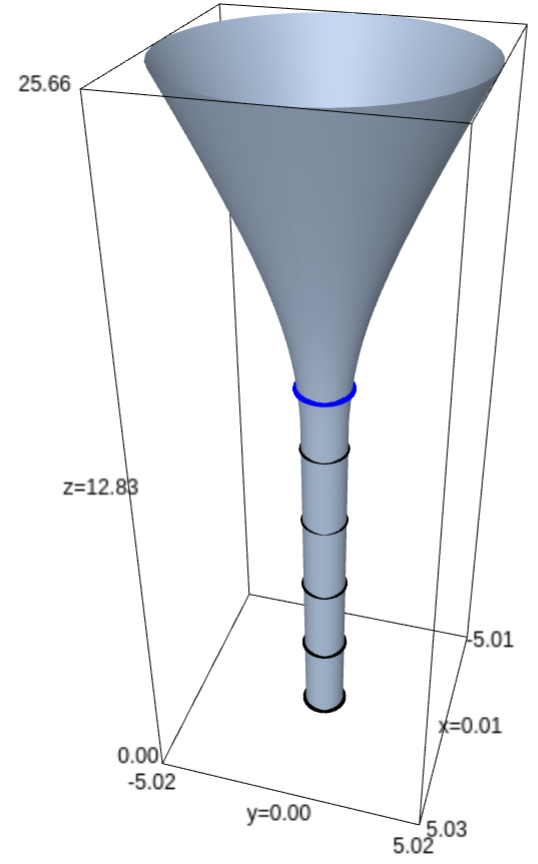
\includegraphics[width=0.35\textwidth]{exk_throat_emb_pi6.png}
}
\caption[]{\label{f:exk:throat_emb} \footnotesize
Isometric embeddings of slices $\Sigma_{t,\th}$ of constant Boyer-Lindquist time $t$
and constant $\th$ of the extremal Kerr spacetime in the Euclidean 3-space,
for two values of $\th$: $\th=\pi/2$ (equatorial plane) (left figure)
and $\th=\pi/6$ (right figure). The slices at truncated at
$r=(1 + 10^{-5})m$ (bottom boundary, for which $z=0$ by convention) and at $r=10\, m$
(top boundary). The blue circle marks the ergosphere, which is located at
$r=2m$ for $\th=\pi/2$ and $r=3m/2$ for $\th=\pi/6$. The five black circles
correspond to $r = 1.1\, m$, $1.01\, m$, $1.001\, m$, $1.0001\, m$
and $1.00001\, m$, from the top to the bottom.
\textsl{[Figure generated by the notebook \ref{s:sam:Kerr_extremal_throat_emb}]}
}
\end{figure}

The functions $\varpi(r)$ and $z(r)$ provided respectively by Eqs.~(\ref{e:exk:isom_emb_cond1})
and (\ref{e:exk:isom_emb_z_r}) define fully the isometric embedding
(\ref{e:exk:isom_emb_z_r}) of $(\Sigma_{t,\th})$ in $(\R^3,\w{f})$.
The outcome is depicted in Fig.~\ref{f:exk:throat_emb}
for two values of $\th$: $\pi/2$ (left plot) and $\pi/6$ (right plot).
In both cases, it appears that the embedded surface is infinite in two directions:
\begin{itemize}
\item for $r\to +\infty$, which implies $\varpi \to +\infty$ and $z \to +\infty$;
\item for $r\to m$, which implies $\varpi \to 2m\frac{\sin\th}{\sqrt{1 + \cos^2\th}}$ and $z\to -\infty$.
\end{itemize}
The first direction is towards the asymptotic flat end of $\M_{\rm I}$
(the right-most corner in the Carter-Penrose diagram of Fig.~\ref{f:exk:CPdiag_BL}).
The second direction corresponds to an infinite cylinder, since
$\varpi$ tends to a constant value, while $z$ decays to $-\infty$.














